\documentclass[crop,border={2pt 0 2pt 0},tikz]{standalone}
\usepackage{tikz-3dplot}
\usepackage{braket}
\usetikzlibrary{decorations.markings, backgrounds, calc, arrows.meta, bending}
\tikzset{>=latex}
\tikzset{->-/.style={decoration={
    markings,
    mark=at position .5 with {\arrow{>}} },postaction={decorate}}
}

\tikzset{-./.style={decoration={
    markings,
    mark=at position 0.999 with {\pgfuseplotmark{*}} },postaction={decorate}}
}

\tikzset{->-./.style={decoration={
    markings,
    mark=at position 0.6 with {\arrow{>}},
    mark=at position 1 with {\pgfuseplotmark{*}}
    },postaction={decorate}}
}

\tikzset{->->-./.style={decoration={
    markings,
    mark=at position 0.3 with {\arrow{>[bend]}},
    mark=at position 0.8 with {\arrow{>[bend]}},
    mark=at position 0.999 with {\pgfuseplotmark{*}}
    },postaction={decorate}}
}

\tikzset{-<-./.style={decoration={
    markings,
    mark=at position 0.6 with {\arrow{<}},
    mark=at position 1 with {\pgfuseplotmark{*}}
    },postaction={decorate}}
}
\begin{document}
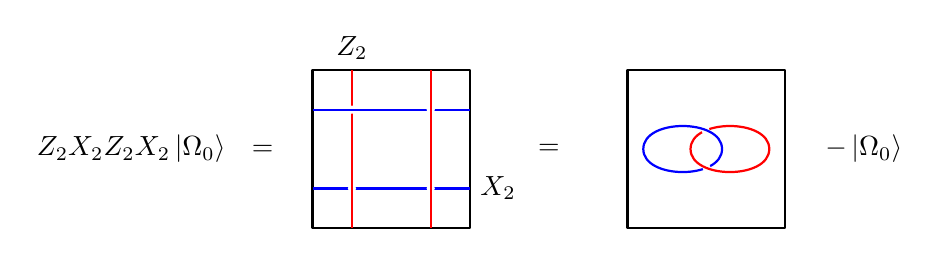
\begin{tikzpicture}[line join = round]

\node[anchor=center] at (-2, 1) {$Z_2 X_2 Z_2 X_2 \ket{\Omega_0} \ \    =$};


\draw[black, thick] (0,0) rectangle (2,2);

\draw[blue, thick](0,0.5) -- node[pos = 0.25, fill=white, anchor=center, circle,inner sep =0pt ,  minimum size= 3pt]{} node[pos = 0.75, fill=white, anchor=center, circle,inner sep =0pt ,  minimum size= 3pt]{} +(2,0) node[anchor=west, black ] {$X_2$};

\draw[red, thick](0.5,0) -- node[pos = 0.75, fill=white, anchor=center, circle,inner sep =0pt ,  minimum size= 3pt]{} +(0,2) node[anchor=south, black ] {$Z_2$};

\draw[blue, thick](0,1.5) -- node[pos = 0.75, fill=white, anchor=center, circle,inner sep =0pt ,  minimum size= 3pt]{} +(2,0);

\draw[red, thick](1.5,0) --  +(0,2);

\node[anchor=center] at (3, 1) {$=$};

\draw[black, thick] (4,0) rectangle (6,2);

\draw[blue, thick](5.2,1) to [out=270, in=270]  node[pos = 0.284, fill=white, anchor=center, circle,inner sep =0pt ,  minimum size= 3pt]  {}  (4.2,1);

\draw[red, thick](5.8,1) to [out=90, in=90] node[pos = 0.72, fill=white, anchor=center, circle,inner sep =0pt ,  minimum size= 3pt]  {}  (4.8,1) to [out=270, in=270] (5.8,1);

\draw[blue, thick](5.2,1) to [out=90, in=90]  (4.2,1);

\node[anchor=center] at (7, 1) {$ - \ket{\Omega_0}$};


% \draw[red, thick]  (4.7, 1)  ellipse (0.45 and 0.7) node[fill=white, anchor=center, circle,inner sep =0pt ,  minimum size= 3pt]{z} ;

% \draw[blue, thick] (5.3, 1) ellipse (0.45 and 0.7); 
% node[pos = 0.1, fill=white, anchor=center, circle,inner sep =0pt ,  minimum size= 3pt]{}
\end{tikzpicture}

\end{document} 
